\documentclass[a4paper, 12pt]{report}
\usepackage[T1]{fontenc}
\usepackage[utf8]{inputenc}
\usepackage[english]{babel}
\usepackage{mathtools}
\usepackage{amsfonts}
\usepackage{amsmath}
\usepackage{mathrsfs}
\usepackage{enumitem}
\usepackage{booktabs}
\usepackage{array}
% Avoid paragraph indent
\setlength{\parindent}{0pt}
% Useful floor and ceiling functions
\DeclarePairedDelimiter{\floor}{\lfloor}{\rfloor}
\DeclarePairedDelimiter{\ceil}{\lceil}{\rceil}
% Modified margins
\usepackage[margin=2cm]{geometry}
% This avoids hypenation
\hyphenpenalty=10000
\usepackage{tikz}
\usetikzlibrary{arrows,calc,positioning,shadows,shapes}
\usepackage{graphicx}
\graphicspath{ {figs/} }
\usepackage{subfig}
\captionsetup[figure]{labelfont={bf},name={Figure},labelsep=period}
\captionsetup[table]{labelfont={bf},name={Table},labelsep=period}

\usepackage{float}


\begin{document}
	
\title{Digital Communications and Laboratory \\ Second Homework}
\author{Faccin Dario, Santi Giovanni}
\date{}
\maketitle

\section*{Setup and presentation}

\subsection*{Exercise 1}

\subsection*{Exercise 2}
A flat fading channel with only one top $h_0(nT_c)$ was studied, assuming a \textit{Rice factor} of k=2 dB and normalized $M_{h_0}$. Moreover, a classical \textit{Doppler Spectrum} with $f_d T_c=40\cdot10^{-5}$ was considered. The schematical model to generate the coefficient $h_0$ of the channel is given in Fig. \ref{Model_2}

\begin{figure}[h]
	\centering
	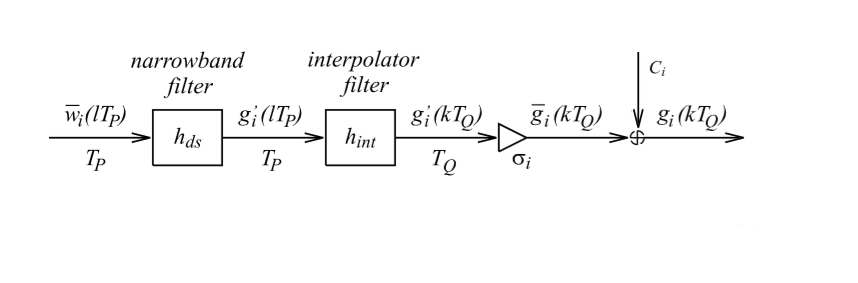
\includegraphics[width=14cm]{images/Model_2}
	\caption{Model to generate the coefficient $h_0$ of the time-varying channel.}\label{Model_2} 
\end{figure}

\section*{Problem 1}

\section*{Problem 2}
To generate the Doppler Spectrum, we used an IIR filter with the following parameters:

\begin{center}
	\begin{table}[h]
		\centering
		\begin{tabular}{c c c c}
			\toprule
			\textbf{$H_{ds}(z) = B(z)/A(z)$} & $f_dT_p=0.1$ &  &     \\
			\midrule
			$\left\lbrace a_n \right\rbrace$ ,& $n=0,\cdots,11$:  & & \\
			1 & -4.4153 & 8.6283 & -9.4592   \\
		    6.1051 & -1.3542 & -3.3622 & 7.2390 \\
		    -7.9361 & 5.1221 & -1.8401 & 2.8706e-1 \\
		    \midrule
		    $\left\lbrace b_n \right\rbrace$ ,& $n=0,\cdots,21$:  & & \\
		    1.3651e-4 & 8.1905e-4 & 2.0476e-3 & 2.7302e-3 \\
		    2.0476e-3 & 9.0939e-4 & 6.7852e-4 & 1.3550e-3 \\
		    1.8076e-3 & 1.3550e-3 & 5.3726e-4 & 6.1818e-5 \\
		    -7.1294e-5 & -9.5058e-5 & -7.1294e-5 & -2.5505e-5 \\
		    1.3321e-5 & 4.5186e-5 & 6.0248e-5 & 4.5186e-5 \\
		    1.8074e-5  & 3.0124e-6  & & \\
		    \bottomrule			
	    \end{tabular}
	\end{table}
\end{center} 

The grafical rapresentation of the impulse resonse of the IIR filter and the Doppler Spectrum is shown in Fig. \ref{DS}. 
To obtain $h_0$, following the scheme of Fig. \ref{Model_2}, the noise component $w\sim \mathcal{CN}(0,1)$ was filtered with the IIR filter previously described. Note that the frequency response of this filter is $H_{ds}(f)=\sqrt{D(f)}$ while the PSD of the noise is constant and equal to 1. For this reason, the equivalent impulse response of this part is equal to $D(f)=1\cdot |H_{ds}|^2$ which is actually the Doppler spectrum. \\
The output of the filter was affected by a transient, which we have avoided by considering only values after $5N_{eq}T_p$, where $N_{eq} = \left\lceil -\frac{1}{\ln(|p|)} \right\rceil$ is the equivalent time constant, and $p$ is the pole with the highest magnitude. Then, after having scaled the coefficient such that $M_{h_0}/\sqrt{E_{h_{ds}}}=1$, the signal was filtered with an interpolation filter of factor $1/T_Q = T_p/T_c=250$. The interpolator output signal was then multiplied by a constant $\sigma_0 = \sqrt{M_d}$ to impose the desired power delay profile, and finally added up with another constant, $C$, which included the deterministic component according to the statistical description of the fading channel.



%Note that the statistical power of $h_0$ is normalized to one.

\begin{figure}[h!]
	\centering
	\subfloat{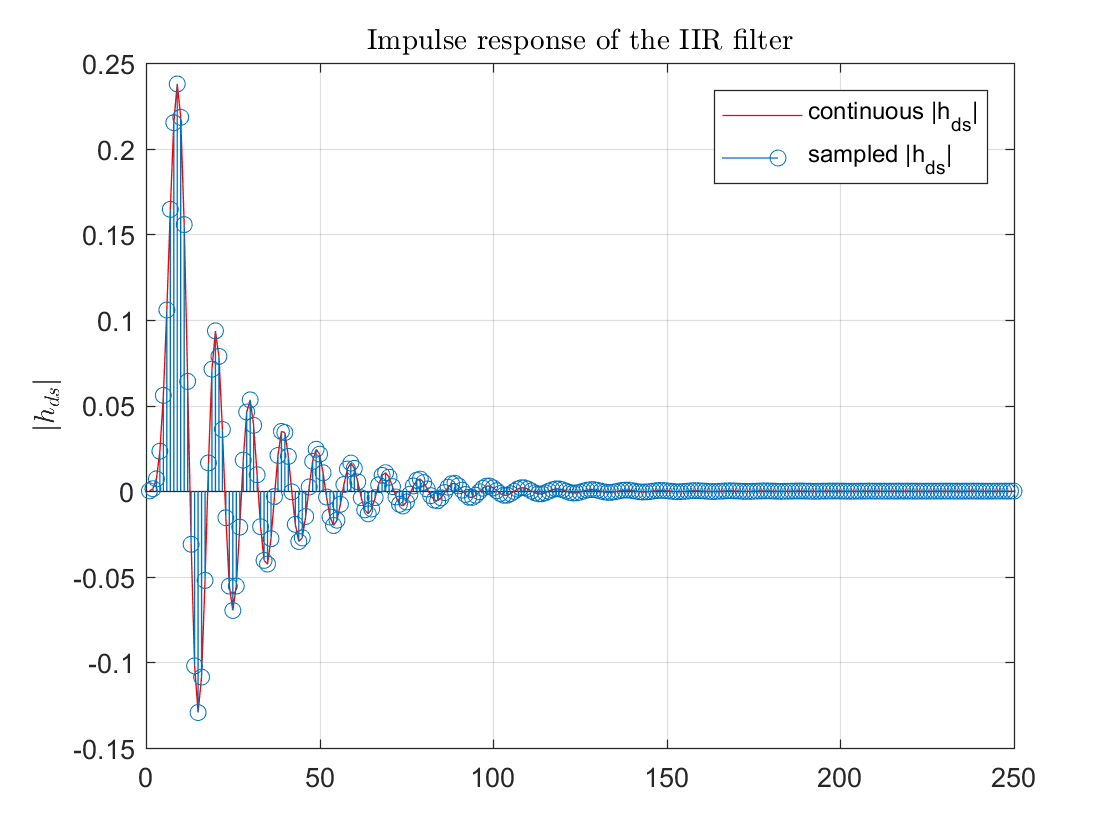
\includegraphics[width=7.5cm]{images/h_d}}
	\subfloat{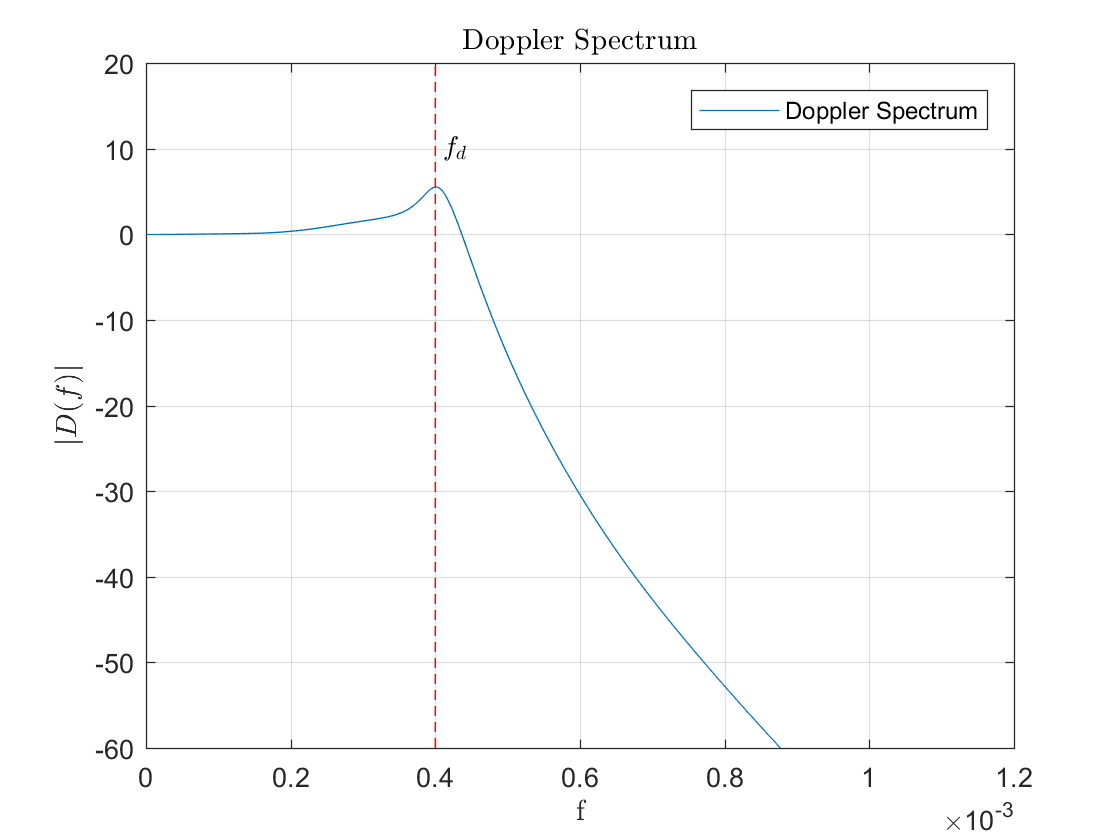
\includegraphics[width=7.5cm]{images/D}}
	\caption{impulse resonse of the IIR filter and 	Doppler Spectrum.}\label{DS}
\end{figure}

\begin{thebibliography}{15}
	\bibitem{nevio<3}
	Nevio Benvenuto, Giovanni Cherubini,
	\textit{Algorithms for Communication Systems and their Applications}. 
	Wiley, 2002.
\end{thebibliography}

\end{document}